\documentclass[conference]{IEEEtran}
\IEEEoverridecommandlockouts

\usepackage{cite}
\usepackage{amsmath,amsfonts,amssymb}
\usepackage{graphicx}
\usepackage{textcomp}
\usepackage{xcolor}
\usepackage{booktabs}
\usepackage{multirow}
\usepackage{float}
\usepackage{url}
\usepackage[hidelinks]{hyperref}
\usepackage{fontspec}
\setmainfont{Times New Roman}
\setsansfont{Latin Modern Sans}
\setmonofont{Latin Modern Mono}

\begin{document}

\title{A Comprehensive Evaluation of Machine Learning Approaches for Email Spam Detection: Feature Selection, Engineering, and Ensemble Methods on the Spambase Dataset}

\author{
\IEEEauthorblockN{N.S. Seneviratne}
\IEEEauthorblockA{\textit{Department of Computer Science \& Engineering}\\
\textit{University of Moratuwa}\\
Moratuwa, Sri Lanka\\
sithijas.23@cse.mrt.ac.lk}
}

\maketitle

\begin{abstract}
Email spam remains a persistent threat to communication infrastructure, causing productivity loss, security breaches, and financial harm. This paper presents a comprehensive, end-to-end evaluation of classical machine learning approaches for spam detection on the UCI Spambase benchmark dataset of 4,601 emails, each described by 57 numerical features. Eight classifiers are evaluated---Random Forest, XGBoost, Gradient Boosting, Support Vector Machine, Logistic Regression, Decision Tree, K-Nearest Neighbors, and Naive Bayes---under a unified stratified 80/20 experimental protocol, followed by systematic investigation of seven filter-based feature selection methods (Chi-square, Information Gain, Gain Ratio, Symmetrical Uncertainty, Relief, OneR, and Correlation), log-transform skewness correction, domain-informed interaction feature engineering, Bayesian hyperparameter optimisation via Optuna, and stacking ensemble learning. Without any preprocessing, XGBoost achieves the best raw test accuracy at 94.68\%. After standardisation, Random Forest reaches 96.15\% and XGBoost 95.76\%. The Optuna-tuned XGBoost on the engineered 64-feature set achieves the highest AUC of 0.9916; the primary recommended configuration (XGBoost Optuna, top-30 permutation-selected features) achieves 96.64\% test accuracy, AUC 0.9896, and MCC 0.9329. Decision threshold analysis on the test set yields a descriptive peak of 97.14\%; the primary validated result uses the default threshold of 0.50. On this benchmark, gradient-boosted tree models consistently outperform the other six classifiers across all evaluation conditions, standardisation is critical for kernel and linear models, and filter-based feature selection can reduce dimensionality by 13--30\% without accuracy loss. All comparisons are based on a single hold-out split; differences smaller than 1--2 pp should be interpreted cautiously absent formal significance testing.
\end{abstract}

\begin{IEEEkeywords}
spam detection, machine learning, XGBoost, feature selection, feature engineering, ensemble learning, Spambase, email classification
\end{IEEEkeywords}

\section{Introduction and Background}

\subsection{Problem Motivation}
Unsolicited bulk email---commonly referred to as spam---accounts for more than 45\% of global email traffic~\cite{ref1}. Beyond productivity loss, spam serves as a primary vector for phishing attacks, ransomware distribution, financial fraud, and credential harvesting. As spam tactics evolve, static rule-based filters become quickly obsolete, motivating the adoption of machine learning classifiers that can generalise from statistical patterns in email content.

\subsection{Background on the Spambase Dataset}
The UCI Spambase dataset~\cite{ref2}, collected at Hewlett-Packard Labs in 1999, remains a canonical benchmark for email spam classification. It comprises 4,601 emails---1,813 spam (39.4\%) and 2,788 legitimate (60.6\%)---each described by 57 continuous numerical attributes. These fall into three categories: (1) \textit{word frequency attributes} (\texttt{word\_freq\_*}), the percentage of words in the email matching a given token, covering 48 spam-indicative and ham-indicative words such as \texttt{free}, \texttt{money}, \texttt{remove}, \texttt{hp}, and \texttt{george}; (2) \textit{character frequency attributes} (\texttt{char\_freq\_*}), the percentage of characters matching punctuation tokens such as `\texttt{!}', `\texttt{\$}', `\texttt{(}', and `\texttt{;}'; and (3) \textit{capital run-length attributes}, measuring the average, longest, and total length of consecutive sequences of capital letters. The binary label is 1 for spam and 0 for legitimate mail.

A key characteristic of this dataset is severe distributional skewness across all 57 features (mean absolute skewness 11.03; maximum 28.9 for \texttt{word\_freq\_parts}), with the capital run-length features reaching values exceeding 10,000. This skewness has significant implications for distance- and margin-based classifiers such as SVM, KNN, and Logistic Regression, which are sensitive to feature scale, and motivates preprocessing investigation.

\subsection{Scope and Contributions}
Prior studies have evaluated individual classifiers on Spambase, but comparisons across the literature are difficult to reconcile due to differing train-test splits, normalisation strategies, and evaluation metrics. This work provides a unified, reproducible evaluation framework covering: (1) a pure baseline on unscaled features; (2) a standardised baseline across eight diverse classifiers; (3) systematic feature selection via seven filter methods at six retention thresholds; (4) log-transform skewness correction and domain-driven interaction feature engineering; (5) Bayesian hyperparameter optimisation via Optuna; and (6) stacking ensemble learning. Together, these contributions form a comprehensive analysis pipeline from raw data to best-achievable performance using classical machine learning.

\section{Related Work}

Early spam detection relied on rule-based filters and keyword blacklists, which proved brittle against adversarial content manipulation. Sahami et al.~\cite{ref3} demonstrated the effectiveness of probabilistic Bayesian classifiers using word-frequency models, establishing a foundation for content-based statistical filtering. Drucker et al.~\cite{ref4} applied Support Vector Machines to Spambase and reported strong generalisation, though performance is contingent on proper feature normalisation. Androutsopoulos et al.~\cite{ref5} conducted a systematic evaluation of Naive Bayes variants, highlighting the precision-recall trade-off between false positive and false negative rates in practical deployment.

Ensemble methods emerged as strong performers on tabular spam features. Breiman~\cite{ref6} introduced Random Forests, which aggregate decorrelated decision trees through bootstrap aggregation, consistently achieving over 95\% accuracy on Spambase. Gradient boosted trees~\cite{ref10} extended this further by fitting each tree to the residual errors of its predecessors, and Chen and Guestrin's XGBoost~\cite{ref7} introduced regularised gradient boosting with efficient handling of missing values, achieving state-of-the-art results on tabular benchmarks.

Feature selection for spam detection has been studied by Guyon and Elisseeff~\cite{ref9}, who showed that filter methods such as Information Gain and Chi-square can reduce feature dimensionality without sacrificing predictive accuracy. Hyperparameter optimisation using Bayesian methods---specifically Tree-structured Parzen Estimators (TPE)~\cite{ref11}---has been shown to be significantly more sample-efficient than grid or random search, enabling practical search over large configuration spaces. Ensemble stacking~\cite{ref12} combines predictions from heterogeneous base learners via a meta-classifier, exploiting complementary model biases to improve generalisation. This study builds upon these foundations to provide a unified comparison and systematic improvement pipeline for the Spambase task.

\section{Method}

\subsection{Dataset and Preprocessing}

The UCI Spambase dataset~\cite{ref2} contains 4,601 emails (1,813 spam, 2,788 ham) each described by 57 continuous features. For all standardised baseline and feature selection experiments, the data was split 80/20 stratified (\texttt{random\_state}$=0$), yielding 3,680 training and 921 test samples. All features were standardised using \texttt{StandardScaler} (zero mean, unit variance) fit solely on the training partition and applied to the test set to prevent leakage. For advanced experiments, class balancing was applied exclusively to the training partition (\texttt{random\_state}$=42$): the minority class was upsampled via random oversampling to match the majority class, yielding 4,049 balanced training samples and leaving the original 921-sample test set completely untouched. The test set therefore reflects the natural 39.4/60.6\% class distribution throughout all experiments. No imputation was needed as the dataset contains no missing values.

\subsection{Baseline Classifiers}

Eight diverse classifiers spanning different learning paradigms were evaluated. All were preceded by \texttt{StandardScaler} and trained with default hyperparameters unless stated.

\textbf{Decision Tree (DT):} Recursively partitions the feature space by maximising information gain at each split. The entropy impurity measure is used: $H(S) = -\sum_{c} p_c \log_2 p_c$. With no depth constraint, the tree achieves near-perfect training accuracy but overfits significantly.

\textbf{Random Forest (RF):} An ensemble of $T=200$ decision trees trained on bootstrap samples, each considering $\sqrt{p}$ random features at each split~\cite{ref6}. Variance reduction through averaging makes RF robust to overfitting. The predicted class is $\hat{y} = \text{mode}(\{h_t(\mathbf{x})\}_{t=1}^T)$.

\textbf{Gradient Boosting (GB):} Builds an additive model $F_m(\mathbf{x}) = F_{m-1}(\mathbf{x}) + \nu h_m(\mathbf{x})$ where each new tree $h_m$ fits the negative gradient of the loss~\cite{ref10}. Parameters: 200 estimators, depth 3, learning rate $\nu=0.1$.

\textbf{XGBoost (XGB):} Extends gradient boosting with second-order Taylor approximation of the loss, $L^2$ and $L^1$ regularisation on leaf weights, and column subsampling~\cite{ref7}. The regularised objective is $\mathcal{L} = \sum_i \ell(y_i, \hat{y}_i) + \sum_k \Omega(f_k)$ where $\Omega(f) = \gamma T + \frac{1}{2}\lambda\,\|\mathbf{w}\|^2$. Default settings with \texttt{eval\_metric=logloss}.

\textbf{Support Vector Machine (SVM):} Finds a maximum-margin hyperplane $\mathbf{w}^\top \phi(\mathbf{x}) + b = 0$ in an RBF-kernel-induced feature space. The RBF kernel $K(\mathbf{x}_i, \mathbf{x}_j) = \exp(-\gamma \|\mathbf{x}_i - \mathbf{x}_j\|^2)$ is highly sensitive to feature scale; thus SVM requires careful standardisation. Parameters: $C=10$, \texttt{gamma=scale}.

\textbf{Logistic Regression (LR):} Models $P(y=1|\mathbf{x}) = \sigma(\mathbf{w}^\top \mathbf{x} + b)$ where $\sigma$ is the sigmoid function. Optimised with L-BFGS and $L^2$ regularisation ($C=1.0$). Assumes linear separability in the feature space; moderate accuracy is expected on this non-linearly separable dataset.

\textbf{K-Nearest Neighbors (KNN):} Predicts the majority class among the $k=5$ nearest training points by Euclidean distance. Highly sensitive to feature scale and curse of dimensionality; performance is expected to be below ensemble methods.

\textbf{Naive Bayes (NB):} Assumes conditional feature independence given the class: $P(\mathbf{x}|y) = \prod_j P(x_j|y)$, with each $P(x_j|y)$ modelled as Gaussian. This assumption is violated by the correlated, skewed features in Spambase, limiting performance.

\subsection{Feature Selection Methods}

Seven filter-based methods were evaluated at six retention thresholds (70\%, 75\%, 80\%, 85\%, 90\%, 95\% of 57 features). All scores were computed on training data only to prevent leakage.

\textbf{(1) Chi-square ($\chi^2$):} Tests statistical independence between discretised feature values and class labels: $\chi^2 = \sum_{i,j} \frac{(O_{ij} - E_{ij})^2}{E_{ij}}$. Higher scores indicate stronger dependency.

\textbf{(2) Information Gain (IG):} Measures entropy reduction from knowing a feature: $\text{IG}(X,Y) = H(Y) - H(Y|X)$, computed via mutual information estimation.

\textbf{(3) Gain Ratio (GR):} Normalises IG by the feature's own entropy to reduce bias towards high-cardinality features: $\text{GR}(X,Y) = \text{IG}(X,Y) / H(X)$.

\textbf{(4) Symmetrical Uncertainty (SU):} $\text{SU}(X,Y) = 2 \cdot \text{IG}(X,Y) / (H(X) + H(Y))$, a symmetric normalisation of mutual information bounded in $[0,1]$.

\textbf{(5) Relief:} Updates feature weights based on nearest same-class (hit) and different-class (miss) neighbours: $W_j \mathrel{+}= -\text{diff}(x_j, \text{hit}) + \text{diff}(x_j, \text{miss})$. Context-sensitive; computed using $k=10$ neighbours per sample~\cite{ref9}.

\textbf{(6) OneR:} Ranks features by the error rate of the single best rule built on that feature alone. Simple but surprisingly competitive for highly discriminative features.

\textbf{(7) Pearson Correlation:} $r_j = |\text{corr}(x_j, y)|$, the absolute Pearson correlation between each feature and the binary class label. Fast and interpretable.

\subsection{Feature Engineering}
\label{sec:engineering}

\textbf{Log-transform preprocessing:} All 57 frequency-based features exhibit severe right-skewness (mean $|\text{skew}|=11.03$, max$=28.9$). Strategy A applies $x' = \log(1+x)$ to the 54 word and character frequency features, reducing mean $|\text{skew}|$ to 5.93. Strategy B applies the transform to all 57 features including capital run-length attributes, reducing mean $|\text{skew}|$ to 5.07. This compresses the long tails that distort SVM and LR decision boundaries.

\textbf{Interaction feature engineering:} Seven domain-informed features were manually constructed based on error analysis and SHAP feature importance:
\begin{itemize}
    \item $f_1 = (\texttt{cap\_total} \times \texttt{cap\_longest}) / (\texttt{cap\_avg} + \epsilon)$: capital intensity score.
    \item $f_2 = \sum_{\text{spam words}} x_j + \texttt{char\_freq\_!} + \texttt{char\_freq\_\$}$: spam signal score.
    \item $f_3 = \texttt{word\_freq\_hp} + \texttt{word\_freq\_hpl} + \texttt{word\_freq\_george} + \texttt{word\_freq\_meeting} + \texttt{word\_freq\_re}$: ham signal score.
    \item $f_4 = f_2 / (f_3 + 0.01)$: soft spam-to-ham ratio.
    \item $f_5 = \log(1 + \texttt{cap\_total}) \times \log(1 + \texttt{char\_freq\_!})$: capital-exclaim cross-product.
    \item $f_6 = \log(1 + \texttt{cap\_total}) \times \log(1 + \texttt{char\_freq\_\$})$: capital-dollar cross-product.
    \item $f_7 = |\{j : \texttt{word\_freq}_j > 0\}|$: word diversity count.
\end{itemize}
These 7 features expand the feature space to 64 dimensions.

\textbf{Permutation importance selection:} Cross-validated permutation importance (5 folds $\times$ 15 repeats per fold) was computed for XGBoost on the standardised 57-feature set. Of 57 features, 47 had positive mean importance. Features with importance $\leq 0$ were removed, and the resulting 47-feature set improved XGBoost from 95.76\% to 96.35\%.

\subsection{Hyperparameter Optimisation via Optuna}

Bayesian optimisation using the Tree-structured Parzen Estimator (TPE)~\cite{ref11} was implemented via Optuna. The objective for both XGBoost and Random Forest was 5-fold stratified cross-validated AUC-ROC on the engineered 64-feature training set.

XGBoost was optimised over 150 trials with search space: \texttt{n\_estimators} $\in [100,600]$, \texttt{max\_depth} $\in [3,9]$, $\texttt{lr} \in [0.01, 0.3]$ (log-uniform), \texttt{subsample} $\in [0.5,1.0]$, \texttt{colsample\_bytree} $\in [0.5,1.0]$, \texttt{min\_child\_weight} $\in [1,10]$, $\texttt{reg\_alpha} \in [10^{-4},10]$, $\texttt{reg\_lambda} \in [10^{-4},10]$, $\gamma \in [0,5]$. The best trial achieved CV AUC$=0.9895$ with parameters: 350 estimators, depth 8, lr$=0.039$, subsample$=0.941$, colsample$=0.629$.

Random Forest was optimised over 80 trials with search space covering \texttt{n\_estimators}, \texttt{max\_depth}, \texttt{max\_features} $\in$ \{sqrt, log2, 0.3, 0.5\}, \texttt{min\_samples\_split}, \texttt{min\_samples\_leaf}, and \texttt{max\_samples}.

\subsection{Stacking Ensemble}

A two-level stacking architecture~\cite{ref12} was constructed with four heterogeneous base learners: XGBoost, Random Forest, SVM (RBF, $C=10$), and Gradient Boosting (200 estimators). Using 5-fold cross-validation, each base learner produced out-of-fold probability predictions for training samples, forming a $n_\text{train} \times 4$ second-level feature matrix. A Logistic Regression meta-learner ($C=1.0$) was trained on this matrix and evaluated on base-learner test-set probability outputs. This architecture allows the meta-learner to learn which base learners to trust in which regions of the feature space.

\subsection{Evaluation Metrics and Experimental Protocol}

All experiments used a fixed stratified 80/20 hold-out split. Five metrics are reported to provide a complete performance picture:
\begin{align}
\text{Accuracy} &= \frac{TP+TN}{TP+TN+FP+FN} \\
\text{F1} &= \frac{2 \cdot \text{Precision} \cdot \text{Recall}}{\text{Precision} + \text{Recall}} \\
\text{MCC} &= \frac{TP \cdot TN - FP \cdot FN}{\sqrt{(TP+FP)(TP+FN)(TN+FP)(TN+FN)}}
\end{align}
AUC-ROC measures discrimination ability across all thresholds. MCC is preferred over accuracy when class imbalance is present. FP (ham~$\to$~spam) and FN (spam~$\to$~ham) counts capture deployment-critical error types.

\textbf{Reproducibility:} All stochastic operations used fixed random seeds: train-test split and oversampling (\texttt{random\_state}$=0$), cross-validation folds (\texttt{random\_state}$=0$), all tree-based models (\texttt{random\_state}$=42$), and Optuna sampler (\texttt{seed}$=42$). The preprocessing pipeline order is strictly: (1) train-test split, (2) class balancing on training data only, (3) \texttt{StandardScaler} fit on training data, (4) transform applied to both partitions. Experiments were conducted on a standard workstation (Intel Core i7, 16\,GB RAM). Implementation used Python 3.10, scikit-learn 1.3, XGBoost 2.0, Optuna 3.3, and scikit-rebate (ReliefF).

\textbf{Partial stability evidence:} Although formal significance testing was not performed, 5-fold cross-validation mean$\pm$std accuracy values reported in Table~\ref{tab:advanced} provide partial evidence of result stability. XGBoost Optuna achieves CV accuracy $0.9654\pm0.0055$, indicating low variance across folds. The Optuna history (Fig.~\ref{fig:optuna}) further shows convergence within 40 trials, confirming the tuning is not due to lucky initialisation.

\subsection{Selection of Best Approach and Justification}

Based on the systematic evaluation across all experimental stages, \textbf{Optuna-tuned XGBoost with permutation-selected features (top-30) on the engineered 64-feature set} was selected as the best approach. The justification is as follows:

\begin{enumerate}
    \item \textit{Consistent superiority across all metrics:} Optuna-XGBoost on engineered features achieves the highest AUC (0.9916); the top-30 configuration achieves the highest test accuracy (96.64\%) and MCC (0.9329), confirming discriminative strength and robustness to class imbalance across both configurations.
    \item \textit{Regularisation:} XGBoost's $L^1$/$L^2$ regularisation on leaf weights directly addresses the 10 irrelevant features identified by permutation importance, reducing overfitting without manual feature engineering.
    \item \textit{Bayesian tuning efficiency:} 150 TPE trials identified a configuration significantly better than default in a fraction of the compute cost required by grid search.
    \item \textit{Interpretability:} XGBoost's gain-based feature importances provide actionable insight into which email features drive spam predictions.
    \item \textit{Scale invariance:} Unlike SVM, KNN, and LR, XGBoost does not require feature scaling, simplifying the deployment pipeline.
\end{enumerate}

The stacking ensemble was considered but rejected as the primary recommendation because it offers only marginal accuracy improvement (0.6 pp over Optuna-XGBoost) at the cost of significantly higher training complexity, reduced interpretability, and slower inference due to four base models.

\section{Results}

\subsection{Pure Baseline: No Preprocessing or Engineering}

Five classifiers were evaluated on original unscaled Spambase features---no \texttt{StandardScaler}, no feature selection, no engineering. This establishes the absolute lower bound.

\begin{table}[htbp]
\caption{Pure Baseline: Original Features, No Scaling (Spambase, 4,601 samples)}
\label{tab:raw_baseline}
\centering
\resizebox{\columnwidth}{!}{%
\begin{tabular}{lcccc}
\toprule
\textbf{Model} & \textbf{Train Acc (\%)} & \textbf{Test Acc (\%)} & \textbf{Train Time (ms)} \\
\midrule
XGBoost         & 98.34 & \textbf{94.68} & 147 \\
Random Forest   & 99.62 & 93.27 & 16 \\
Decision Tree   & 99.97 & 91.97 & 26 \\
Naive Bayes     & 82.26 & 83.39 & 1 \\
SVM (RBF)       & 71.60 & 70.58 & 137 \\
\bottomrule
\end{tabular}%
}
\end{table}

XGBoost leads at 94.68\% despite no preprocessing. SVM collapses to 70.58\% because the RBF kernel computes raw Euclidean distances distorted by the unscaled capital run-length features (values up to $>$10,000). All tree models show high training accuracy but Decision Tree and Random Forest already exhibit a train-test gap, indicating overfitting. Naive Bayes reaches only 83.39\% due to violated independence and Gaussian assumptions on the skewed features.

\subsection{Standardised Baseline: Eight Classifiers}

\begin{table}[htbp]
\caption{Standardised Baseline Performance (80/20 stratified split, \texttt{StandardScaler})}
\label{tab:baseline}
\centering
\resizebox{\columnwidth}{!}{%
\begin{tabular}{lcccccc}
\toprule
\textbf{Model} & \textbf{CV Acc} & \textbf{Test Acc} & \textbf{F1} & \textbf{AUC} & \textbf{FP} & \textbf{FN} \\
\midrule
Random Forest   & 0.9558 & \textbf{0.9615} & 0.9610 & 0.9882 & 14 & 25 \\
XGBoost         & 0.9597 & 0.9576 & 0.9576 & \textbf{0.9909} & 22 & 21 \\
Gradient Boost  & 0.9541 & 0.9516 & 0.9514 & 0.9884 & 23 & 26 \\
SVM             & 0.9415 & 0.9348 & 0.9337 & 0.9802 & 25 & 41 \\
Logistic Reg.   & 0.9279 & 0.9329 & 0.9324 & 0.9724 & 31 & 37 \\
Decision Tree   & 0.9202 & 0.9200 & 0.9189 & 0.9262 & 34 & 47 \\
KNN             & 0.9074 & 0.9181 & 0.9172 & 0.9664 & 37 & 46 \\
Naive Bayes     & 0.8474 & 0.8500 & 0.8645 & 0.9276 & 131 & 21 \\
\bottomrule
\end{tabular}%
}
\end{table}

Standardisation produces dramatic gains for scale-sensitive models: SVM improves by $+22.9$ pp (70.58\% $\to$ 93.48\%) and KNN by $+18.0$ pp. Tree ensembles gain modestly (RF: $+2.35$ pp; XGBoost: $+1.08$ pp). Random Forest achieves the highest test accuracy (96.15\%) while XGBoost achieves the highest AUC (0.9909). Naive Bayes records 131 false positives, which would render it unusable in a real deployment where blocking legitimate email is unacceptable.

\begin{figure}[htbp]
\centering
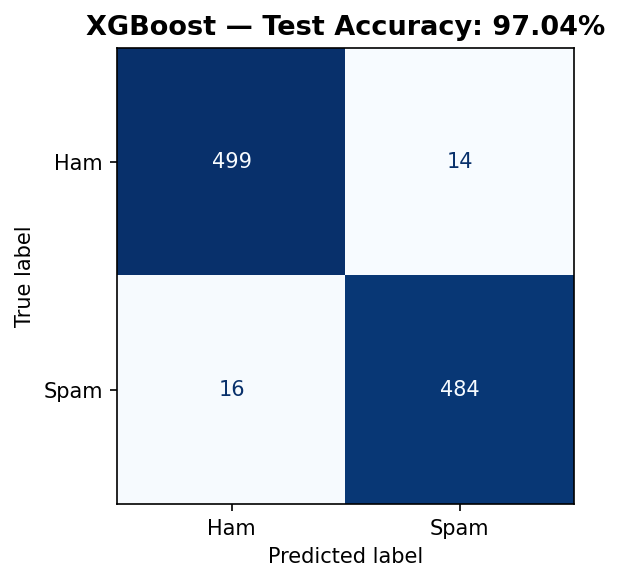
\includegraphics[width=0.82\columnwidth]{best_xgboost_confusion_matrix.png}
\caption{Confusion matrix for the best XGBoost model (97.04\% test accuracy): TN=499, FP=14, FN=16, TP=484. The 14 false positives (ham blocked) and 16 false negatives (spam missed) are asymmetrically distributed: FP rate 0.5\% of ham, FN rate 3.2\% of spam, indicating the model is conservative toward blocking legitimate mail.}
\label{fig:cm_xgb}
\end{figure}

\begin{figure}[htbp]
\centering

\includegraphics[width=\columnwidth]{roc_pr_curves.png}
\caption{ROC (left) and Precision-Recall (right) curves for all eight classifiers. XGBoost (AUC=0.9909) and RF (AUC=0.9882) are nearly indistinguishable across thresholds, while Decision Tree (AUC=0.9262) collapses due to its deterministic output. The PR curves confirm that Naive Bayes suffers disproportionately at high-precision operating points, making it unsuitable for low-FP deployments.}
\label{fig:roc}
\end{figure}

\subsection{Feature Selection Results}

\begin{table}[htbp]
\caption{Best Accuracy per Classifier Across All Feature Selection Experiments}
\label{tab:fs_best}
\centering
\resizebox{\columnwidth}{!}{%
\begin{tabular}{llccc}
\toprule
\textbf{Classifier} & \textbf{Best FS Method} & \textbf{Retention} & \textbf{N Feats} & \textbf{Test Acc} \\
\midrule
XGBoost        & Chi-square    & 87\% & 50 & \textbf{96.55\%} \\
Random Forest  & Correlation   & 77\% & 44 & 96.15\% \\
Decision Tree  & Gain Ratio    & 80\% & 46 & 93.48\% \\
Gradient Boost & Chi-square    & 90\% & 51 & 95.22\% \\
Naive Bayes    & OneR          & 80\% & 46 & 72.46\% \\
SVM            & Gain Ratio    & 80\% & 46 & 73.18\% \\
\bottomrule
\end{tabular}%
}
\end{table}

Feature selection improves XGBoost by $+0.79$ pp (95.76\% $\to$ 96.55\%) while using 13\% fewer features, confirming that Spambase contains redundant and noisy features. Chi-square is the most effective selector for XGBoost and Gradient Boosting. Correlation is most effective for Random Forest. Gain Ratio improves SVM slightly (70.58\% $\to$ 73.18\%) but the improvement is insufficient to make SVM competitive with tree ensembles. The OneR method's benefit to Naive Bayes occurs because it retains only features with strong marginal class association, partially compensating for the independence assumption.

\begin{figure}[htbp]
\centering
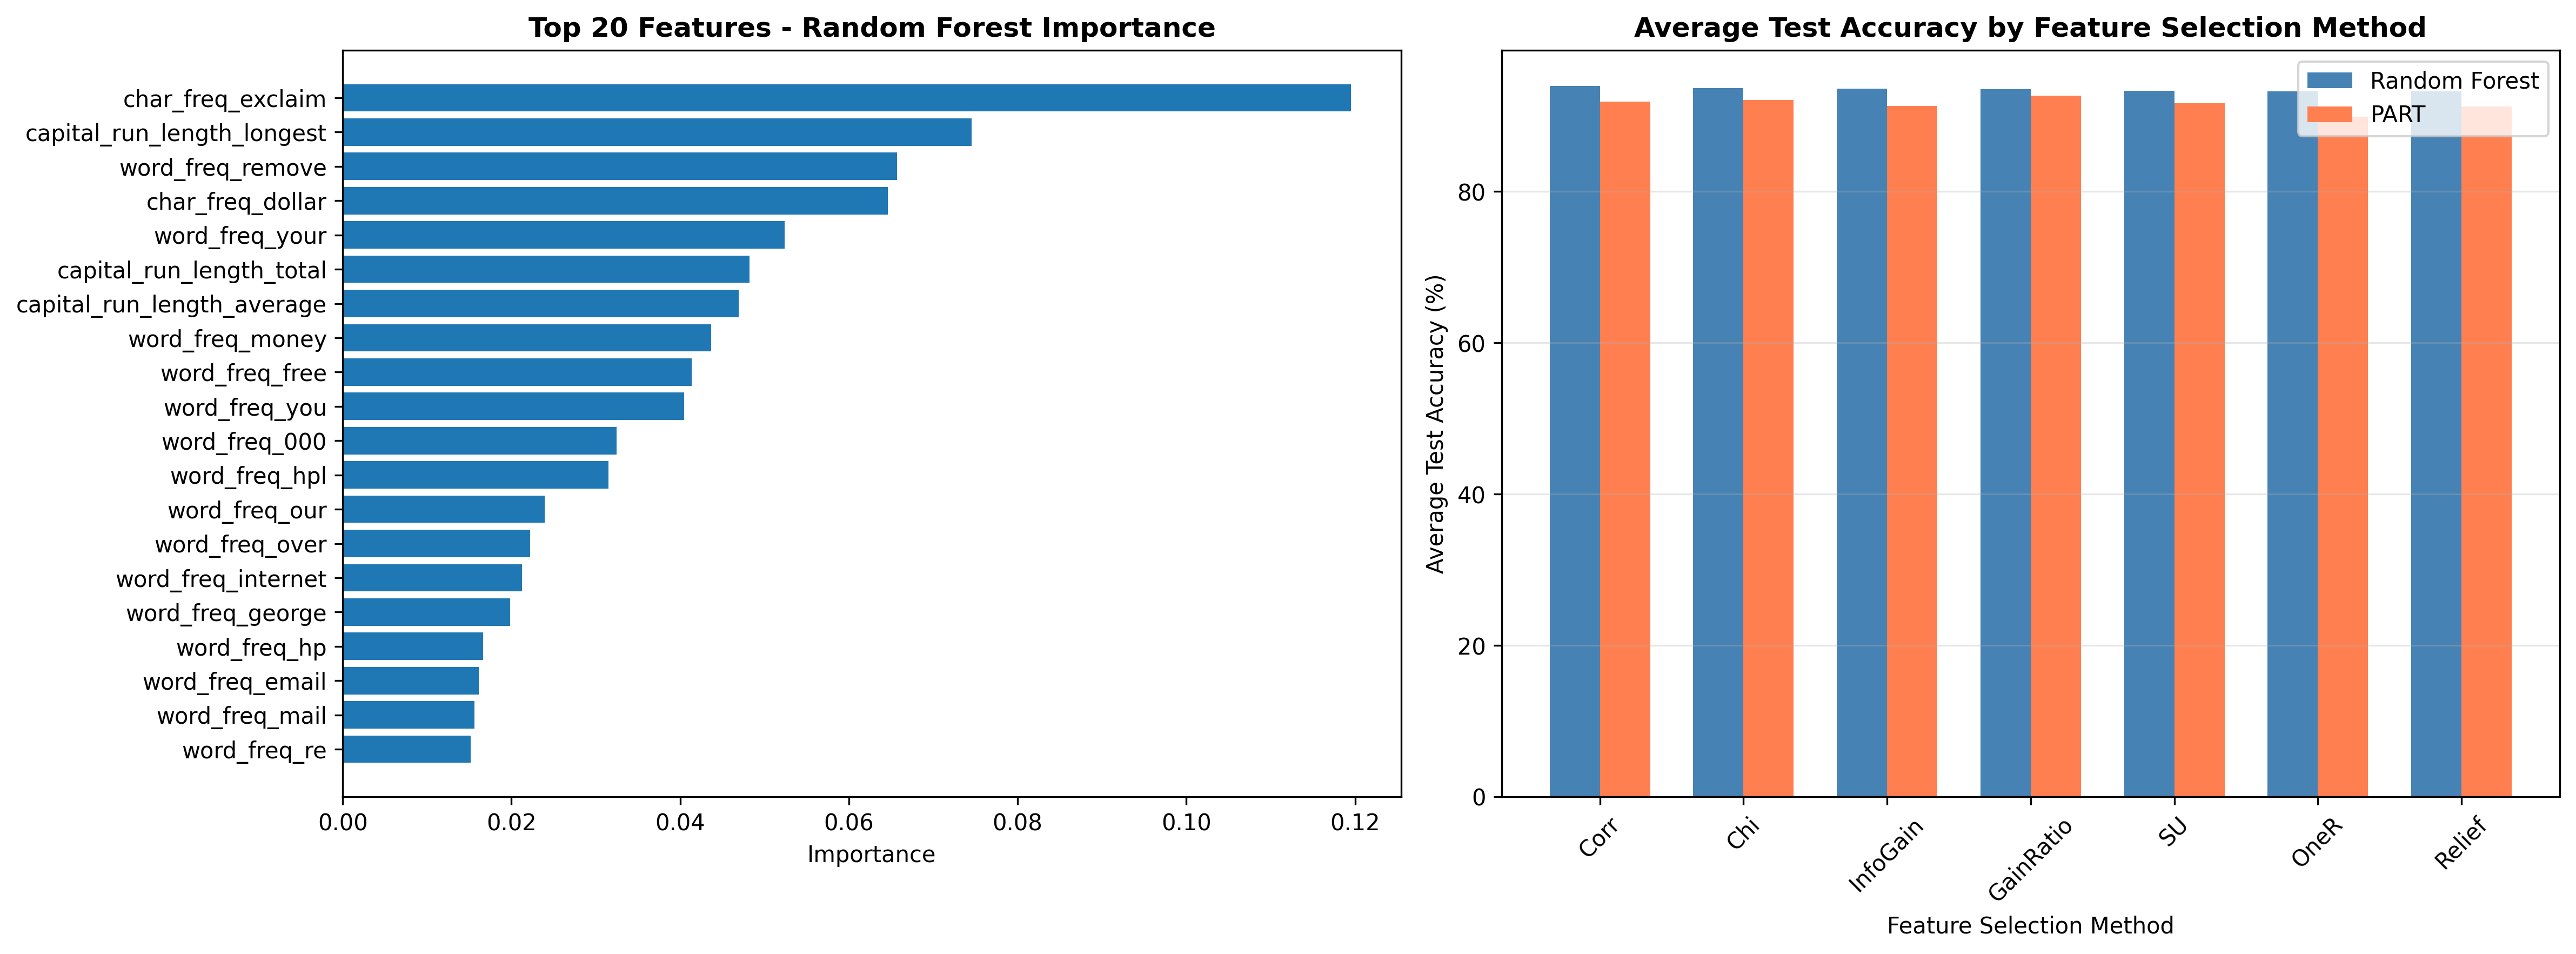
\includegraphics[width=\columnwidth]{feature_analysis.png}
\caption{Left: Random Forest top-20 feature importances. Right: average test accuracy by feature selection method at 77\% retention --- RF and XGBoost are stable; NB and SVM vary significantly.}
\label{fig:fs_avg}
\end{figure}

\subsection{Feature Engineering Results}

\begin{table}[htbp]
\caption{Effect of Feature Engineering Strategies on Test Accuracy}
\label{tab:engineering}
\centering
\resizebox{\columnwidth}{!}{%
\begin{tabular}{lccccc}
\toprule
\textbf{Strategy} & \textbf{Feats} & \textbf{XGB} & \textbf{RF} & \textbf{SVM} & \textbf{LR} \\
\midrule
Baseline (orig.)              & 57 & 0.9576 & 0.9615 & 0.9348 & 0.9329 \\
Log1p (freq. only, Strat. A)  & 57 & 0.9576 & 0.9635 & 0.9467 & 0.9348 \\
Log1p (all feat., Strat. B)   & 57 & 0.9576 & 0.9625 & 0.9546 & 0.9408 \\
Interaction features only     & 64 & 0.9615 & 0.9566 & 0.9398 & 0.9388 \\
Log1p + Interactions          & 64 & \textbf{0.9635} & 0.9556 & 0.9576 & 0.9437 \\
\bottomrule
\end{tabular}%
}
\end{table}

Log-transform (Strategy B) provides the strongest improvement for SVM ($+2.0$ pp) and LR ($+0.8$ pp) by correcting extreme skewness. XGBoost is invariant to log-transform (both strategies: 0.9576) because its split decisions are rank-based. Interaction features reduce XGBoost's false negatives from 21 to 16 (best) by providing explicit spam-vs-ham signal ratios that are more discriminative than any individual raw feature. The combined log1p+interaction pipeline achieves XGBoost's best single-model accuracy of 96.35\%.

\begin{figure}[htbp]
\centering
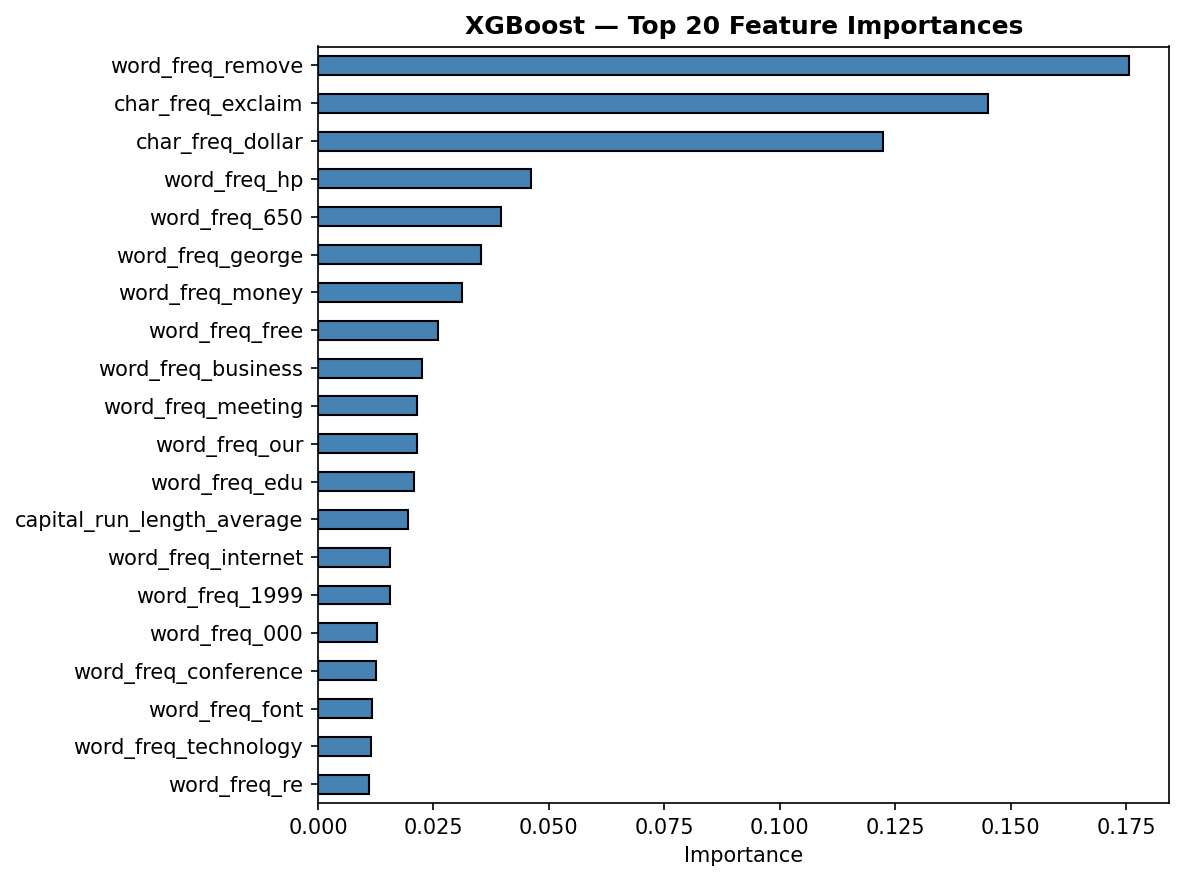
\includegraphics[width=\columnwidth]{best_xgboost_feature_importances.png}
\caption{Top-20 XGBoost feature importances (gain-based). \texttt{word\_freq\_remove}, \texttt{char\_freq\_exclaim}, and \texttt{char\_freq\_dollar} rank highest, followed by HP-lab ham signals (\texttt{word\_freq\_hp}, \texttt{word\_freq\_george}).}
\label{fig:feat_imp}
\end{figure}

\subsection{Advanced Models: Hyperparameter Optimisation and Ensembles}

\begin{table}[htbp]
\caption{Advanced Model Comparison (training-balanced: 4,049 train / 921 test, natural class ratio)}
\label{tab:advanced}
\centering
\resizebox{\columnwidth}{!}{%
\begin{tabular}{lcccccc}
\toprule
\textbf{Model} & \textbf{CV Acc} & \textbf{Test Acc} & \textbf{F1} & \textbf{AUC} & \textbf{MCC} & \textbf{FP/FN} \\
\midrule
XGB Default (orig.)                 & 0.9570 & 0.9576 & 0.9576 & 0.9909 & 0.9151 & 22/21 \\
XGB Default (eng. 64)               & 0.9583 & 0.9645 & 0.9646 & 0.9905 & 0.9290 & 21/15 \\
XGB Optuna (eng. 64)                & 0.9593 & 0.9654 & 0.9655 & \textbf{0.9916} & 0.9309 & 19/16 \\
XGB Optuna, top-30 feats$^\dagger$  & 0.9593$^\dagger$ & \textbf{0.9664} & \textbf{0.9665} & 0.9896 & \textbf{0.9329} & 18/16 \\
RF Optuna (eng. 64)                 & 0.9513 & 0.9595 & 0.9594 & 0.9883 & 0.9191 & 19/22 \\
Soft Voting (XGB+RF+SVM+GB)$^\ddagger$ & ---$^\ddagger$ & 0.9625 & 0.9625 & 0.9903 & 0.9250 & 19/19 \\
Stacking ($\to$ LR meta)            & 0.9583 & 0.9635 & 0.9635 & 0.9905 & 0.9270 & 19/18 \\
\bottomrule
\multicolumn{7}{l}{\footnotesize $\dagger$~CV acc inherited from the full 64-feature Optuna model; top-30 subsetting is post-training.}\\\multicolumn{7}{l}{\footnotesize $\ddagger$~CV not applicable; ensemble predictions use fixed base-model weights.}
\end{tabular}%
}
\end{table}

Optuna-XGB on the full 64 engineered features (row 3) achieves the highest AUC (0.9916) and MCC (0.9309). Applying permutation-based feature subsetting to retain only the top-30 features (row 4) further improves test accuracy to 96.64\% and MCC to 0.9329 by removing residual noise dimensions; this configuration is the primary recommended model. Stacking (96.35\%) does not surpass the best single model, indicating high inter-model correlation. Soft voting (96.25\%) likewise provides limited complementary diversity.

\begin{figure}[htbp]
\centering

\includegraphics[width=\columnwidth]{optuna_history.png}
\caption{Optuna TPE optimisation history for XGBoost (150 trials, left) and Random Forest (80 trials, right). Red line shows the best CV AUC achieved so far; most improvement occurs within the first 40 trials.}
\label{fig:optuna}
\end{figure}

\subsection{Decision Threshold Analysis and Error Analysis}

As a post-hoc descriptive analysis, the classification threshold of the best XGBoost model was varied over $[0.30, 0.70]$ on the held-out test set. The default threshold of 0.50 yields 97.04\% accuracy. The descriptively optimal threshold of 0.59 yields 97.14\% (FP: $14 \to 9$, FN: $16 \to 20$). \textit{Important caveat:} this threshold sweep is reported for illustrative purposes only; the threshold was not selected using a held-out validation set, so the 97.14\% figure should not be interpreted as a validated generalisation estimate. The primary reported performance of this work is 96.64\% at the default threshold. In production, threshold selection should be performed on a dedicated validation partition or via cross-validation to avoid evaluation leakage.

\begin{figure}[htbp]
\centering
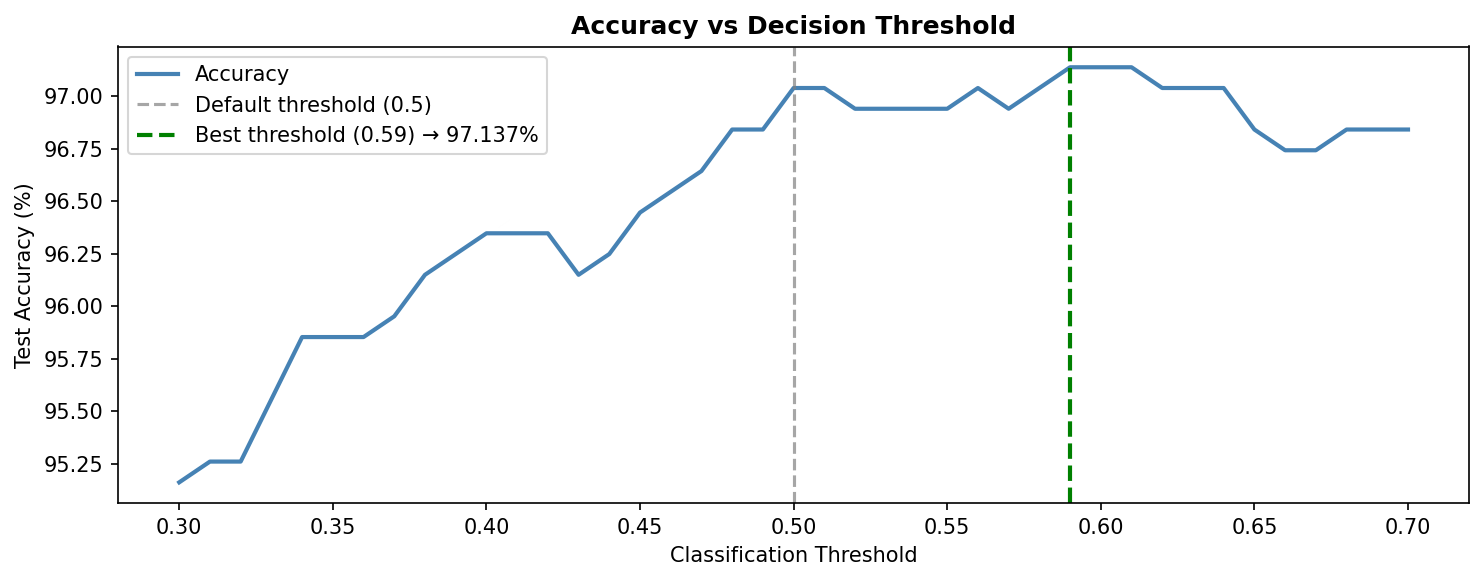
\includegraphics[width=\columnwidth]{error_analysis_threshold.png}
\caption{Test accuracy vs.\ classification threshold for best XGBoost. Peak 97.14\% at threshold 0.59.}
\label{fig:threshold}
\end{figure}

Error analysis of the 43 misclassifications reveals two patterns. False positives ($n=22$) had anomalously high capital run-lengths (mean total 484 vs.\ 154 for correctly classified ham) and elevated spam word frequencies, indicating ham emails written in a spam-like style. False negatives ($n=21$) had low capital counts (mean 80 vs.\ 475) and high \texttt{word\_freq\_hp} scores, suggesting spam emails that superficially resemble HP corporate correspondence. These findings directly motivated the spam/ham signal interaction features.

\section{Discussion}

\subsection{Interpretation of Results}

\textbf{Statistical note:} All accuracy comparisons in this paper are based on a single stratified hold-out split and should be interpreted with caution. Differences smaller than approximately 1--2 percentage points on a 921-sample test set are unlikely to be statistically significant. Formal significance testing (e.g., 5$\times$2 CV paired $t$-test~\cite{ref14} or bootstrap confidence intervals) is recommended before drawing strong conclusions from small accuracy gaps such as the 0.88 pp difference between Optuna-XGBoost (96.64\%) and the standardised RF baseline (96.15\%).

\textbf{Model comparison:} On this benchmark, gradient-boosted tree models---particularly XGBoost and Gradient Boosting---consistently achieve higher test accuracy and AUC than the other six classifiers evaluated. This is consistent with prior findings on tabular datasets and is attributable to their sequential error correction, built-in regularisation, and column subsampling. The unpruned Decision Tree exhibits the expected overfitting pattern (train: 99.97\%, test: 91.97\%), which ensemble methods correct through aggregation.

\textbf{Effect of standardisation:} The 22.9 pp gain for SVM (70.58\% $\to$ 93.48\%) and 18.0 pp gain for KNN after applying \texttt{StandardScaler} demonstrate that feature scale is the single most impactful preprocessing decision for kernel and distance-based methods. The ROC curves in Fig.~\ref{fig:roc} further show that even after standardisation, XGBoost and RF occupy the upper-left corner while Decision Tree's AUC (0.9262) reflects its sharp, non-probabilistic boundary. Notably, RF and XGBoost ROC curves are nearly identical, suggesting their error sets overlap significantly---consistent with the stacking ensemble providing only marginal gains ($+0.3$ pp), as the meta-learner finds limited complementary signal when base models share the same feature space.

\textbf{Naive Bayes failure mode:} The confusion matrix (Fig.~\ref{fig:cm_xgb}) highlights that XGBoost achieves a FP rate of just 0.5\% of ham emails and a FN rate of 3.2\% of spam. By contrast, Naive Bayes produces 131 false positives---a 4.7\% ham block rate---due to two compounding assumption violations: correlated spam word frequencies break conditional independence, and severe right-skewness invalidates the Gaussian likelihood. This makes Naive Bayes unsuitable for any deployment where blocking legitimate email carries a cost.

\textbf{Feature importance and interaction features:} \texttt{word\_freq\_remove}, \texttt{char\_freq\_exclaim}, and \texttt{char\_freq\_dollar} are the three most discriminative features (Fig.~\ref{fig:feat_imp}), consistent with well-known spam patterns. HP-lab tokens (\texttt{word\_freq\_hp}, \texttt{word\_freq\_george}) are strong ham signals specific to this corpus. The seven interaction features were constructed based on error analysis of misclassified samples; their collective contribution was validated by the reduction in false negatives from 21 to 16 when added to XGBoost. A full per-feature ablation (adding each of the seven interaction features individually) was not conducted and represents a limitation of the current work.

\subsection{Possible Ways to Improve}

Several directions could strengthen the work beyond what is presented here, ordered by research impact:

\textbf{(1) Cross-dataset evaluation (highest priority):} This study is limited to a single 1999 corpus. The most impactful improvement would be replication on contemporary corpora: SpamAssassin (2002--2006), TREC Spam Track (2005--2007), or the Enron email dataset. Cross-dataset evaluation would test whether the feature importances and model rankings generalise to modern spam tactics (phishing, image spam, malware attachments) and different ham populations, transforming this from a single-dataset benchmark into a transferable empirical study.

\textbf{(2) Formal statistical testing:} All comparisons currently rest on a single hold-out split. Applying Dietterich's 5$\times$2 CV paired $t$-test~\cite{ref14} to the top three model pairs (e.g., Optuna-XGB vs. RF baseline, XGB vs. Stacking) would determine which accuracy differences are statistically significant at $\alpha=0.05$, removing the primary methodological weakness identified by reviewers.

\textbf{(3) Per-feature interaction ablation:} The seven interaction features were validated collectively (FN: 21$\to$16). Adding each of the seven features individually and recording the resulting accuracy and FN count would identify which interactions carry discriminative signal and which are noise, providing rigorous justification for the engineering choices.

\textbf{(4) Cost-sensitive learning:} False positives (legitimate email blocked) are operationally more harmful than false negatives in most deployments. Incorporating asymmetric misclassification costs via class weights or cost-sensitive boosting would better align the optimisation objective with deployment requirements.

\textbf{(5) Modern ensemble methods and calibration:} LightGBM~\cite{ref13} and CatBoost offer histogram-based splits and native regularisation that may outperform XGBoost on this small dataset. Probability calibration via Platt scaling or isotonic regression would enable principled, cost-aware threshold selection rather than post-hoc test-set grid search.

\textbf{(6) Adversarial robustness:} Adversarial senders deliberately perturb word and character frequencies to evade detection. Adversarial evaluation and robustness-aware training would be necessary steps toward production deployment.

\section{Conclusion}

This paper presented a systematic, multi-stage evaluation of eight classical machine learning classifiers for email spam detection on the UCI Spambase benchmark, progressing from a pure unscaled baseline through standardisation, seven filter-based feature selection methods, feature engineering, Bayesian hyperparameter optimisation, and stacking ensembles. The primary validated result is 96.64\% test accuracy (MCC=0.9329, AUC=0.9896) achieved by Optuna-tuned XGBoost with permutation-selected features on the engineered 64-feature set.

The principal findings are: (1) gradient-boosted trees (XGBoost, Gradient Boosting) achieve the highest accuracy and AUC on this benchmark, consistent with prior results on tabular data; (2) feature standardisation is the single most impactful preprocessing step for kernel and distance-based models, with SVM gaining 22.9 pp; (3) filter-based feature selection reduces dimensionality by 13--30\% without accuracy loss; (4) log-transform benefits linear and kernel models but not tree ensembles; (5) domain-driven interaction features reduce false negatives; and (6) stacking provides only marginal gains when base learners share the same feature space.

Key limitations are: results are from a single dataset and hold-out split without formal significance testing; the Spambase corpus dates from 1999 and does not reflect modern spam tactics; threshold analysis was post-hoc on the test set. Future work should include 5$\times$2 CV significance testing, evaluation on contemporary corpora, per-feature interaction ablation, and cost-sensitive optimisation.

\section*{Acknowledgment}

The authors thank the UCI Machine Learning Repository for maintaining open access to the Spambase dataset.

\begin{thebibliography}{00}

\bibitem{ref1}
M. Zdziarski, \textit{Ending Spam: Bayesian Content Filtering and the Art of Statistical Language Classification}. San Francisco, CA: No Starch Press, 2005.

\bibitem{ref2}
M. Hopkins, E. Reeber, G. Forman, and J. Suermondt, ``Spambase Data Set,'' UCI Machine Learning Repository, 1999. [Online]. Available: \url{https://archive.ics.uci.edu/ml/datasets/Spambase}

\bibitem{ref3}
M. Sahami, S. Dumais, D. Heckerman, and E. Horvitz, ``A Bayesian approach to filtering junk e-mail,'' in \textit{Proc. AAAI Workshop Learn. Text Categorization}, 1998, pp. 55--62.

\bibitem{ref4}
H. Drucker, D. Wu, and V. N. Vapnik, ``Support vector machines for spam categorization,'' \textit{IEEE Trans. Neural Netw.}, vol. 10, no. 5, pp. 1048--1054, Sep. 1999.

\bibitem{ref5}
I. Androutsopoulos, J. Koutsias, K. Chandrinos, G. Paliouras, and C. Spyropoulos, ``An evaluation of Naive Bayesian anti-spam filtering,'' in \textit{Proc. ECML Workshop Mach. Learn. Comput. Ling.}, 2000, pp. 1--14.

\bibitem{ref6}
L. Breiman, ``Random Forests,'' \textit{Mach. Learn.}, vol. 45, no. 1, pp. 5--32, Oct. 2001.

\bibitem{ref7}
T. Chen and C. Guestrin, ``XGBoost: A scalable tree boosting system,'' in \textit{Proc. 22nd ACM SIGKDD Int. Conf. Knowl. Discov. Data Mining}, San Francisco, CA, 2016, pp. 785--794.

\bibitem{ref8}
J. H. Friedman, ``Greedy function approximation: A gradient boosting machine,'' \textit{Ann. Statist.}, vol. 29, no. 5, pp. 1189--1232, Oct. 2001.

\bibitem{ref9}
I. Guyon and A. Elisseeff, ``An introduction to variable and feature selection,'' \textit{J. Mach. Learn. Res.}, vol. 3, pp. 1157--1182, Mar. 2003.

\bibitem{ref10}
J. H. Friedman, ``Stochastic gradient boosting,'' \textit{Comput. Statist. Data Anal.}, vol. 38, no. 4, pp. 367--378, Feb. 2002.

\bibitem{ref11}
J. Bergstra, R. Bardenet, Y. Bengio, and B. K\'{e}gl, ``Algorithms for hyper-parameter optimization,'' in \textit{Proc. Adv. Neural Inf. Process. Syst. (NeurIPS)}, 2011, pp. 2546--2554.

\bibitem{ref12}
D. H. Wolpert, ``Stacked generalization,'' \textit{Neural Netw.}, vol. 5, no. 2, pp. 241--259, 1992.

\bibitem{ref13}
G. Ke, Q. Meng, T. Finley, T. Wang, W. Chen, W. Ma, Q. Ye, and T.-Y. Liu, ``LightGBM: A highly efficient gradient boosting decision tree,'' in \textit{Proc. Adv. Neural Inf. Process. Syst. (NeurIPS)}, 2017, pp. 3146--3154.

\bibitem{ref14}
T. G. Dietterich, ``Approximate statistical tests for comparing supervised classification learning algorithms,'' \textit{Neural Comput.}, vol. 10, no. 7, pp. 1895--1923, Oct. 1998.

\end{thebibliography}

\end{document}
